%%%%%%%%%%%%%%%%%%%%%%%%%%%%%%%%%%%%%%%%%
% Dreuw & Deselaer's Poster
% LaTeX Template
% Version 1.0 (11/04/13)
%
% Created by:
% Philippe Dreuw and Thomas Deselaers
% http://www-i6.informatik.rwth-aachen.de/~dreuw/latexbeamerposter.php
%
% This template has been downloaded from:
% http://www.LaTeXTemplates.com
%
% License:
% CC BY-NC-SA 3.0 (http://creativecommons.org/licenses/by-nc-sa/3.0/)
%
%%%%%%%%%%%%%%%%%%%%%%%%%%%%%%%%%%%%%%%%%

%----------------------------------------------------------------------------------------
%	PACKAGES AND OTHER DOCUMENT CONFIGURATIONS
%----------------------------------------------------------------------------------------

\documentclass[final,hyperref={pdfpagelabels=false}]{beamer}

\usepackage[orientation=portrait,size=a0,scale=1.4]{beamerposter} % Use the beamerposter package for laying out the poster with a portrait orientation and an a0 paper size

\usetheme{I6pd2} % Use the I6pd2 theme supplied with this template

\usepackage[english]{babel} % English language/hyphenation

\usepackage{amsmath,amsthm,amssymb,latexsym} % For including math equations, theorems, symbols, etc

%\usepackage{times}\usefonttheme{professionalfonts}  % Uncomment to use Times as the main font
%\usefonttheme[onlymath]{serif} % Uncomment to use a Serif font within math environments

\boldmath % Use bold for everything within the math environment

\usepackage{booktabs} % Top and bottom rules for tables

\graphicspath{{figures/}} % Location of the graphics files

\usecaptiontemplate{\small\structure{\insertcaptionname~\insertcaptionnumber: }\insertcaption} % A fix for figure numbering

%----------------------------------------------------------------------------------------
%	TITLE SECTION 
%----------------------------------------------------------------------------------------

\title{\huge ESS-NW/CAR} % Poster title

\author{Leon Fernandez, Jonas Ekman, Fredrik Hyyrynen, Jacob Kimblad, Yini Gao and  Yifan Ruan} % Author(s)

\institute{ MF2063 Embedded Systems Design Project} % Institution(s)

%----------------------------------------------------------------------------------------
%	FOOTER TEXT
%----------------------------------------------------------------------------------------

\newcommand{\leftfoot}{ESS-NW/CAR} % Left footer text

\newcommand{\rightfoot}{MF2063} % Right footer text

%----------------------------------------------------------------------------------------

\begin{document}

\addtobeamertemplate{block end}{}{\vspace*{2ex}} % White space under blocks

\begin{frame}[t] % The whole poster is enclosed in one beamer frame

\begin{columns}[t] % The whole poster consists of two major columns, each of which can be subdivided further with another \begin{columns} block - the [t] argument aligns each column's content to the top

\begin{column}{.02\textwidth}\end{column} % Empty spacer column

\begin{column}{.465\textwidth} % The first column


%----------------------------------------------------------------------------------------
%	INTRODUCTION
%----------------------------------------------------------------------------------------
            
\begin{block}{Introduction}

\begin{itemize}
\item This project is about to create an autonomous car that is based on an software-defined network (SDN). On the car is different sensors placed to monitor the performance of the car and all this information is used in a control unit to control the car. The information providers and the consumers have to be connected and this is done via an SDN network there a control unit decides how the packet should be sent via the network. The information providers in the car is ultrasound to measure distance, object recognition and speed sensor. 
\end{itemize}

\end{block}
%
%\begin{block}{Requerments}
%    This is the design requirement for the ESS-CAR
%    \begin{itemize}
%        \item Design and evaluate the software- and system-architecture %for the model car platform. The
%        architecture shall integrate (and potentially adapt) already %existing functionality to achieve a robust and
%        predictable system design.
%
%        \item Setup the physical platform to use different sensors and %actuators (ultrasonic sensor, IR sensor,
%        accelerometer, servo, motor, etc.). The peripherals shall be %controlled with dedicated microcontrollers
%        (Arduino). SPI bus is used to communicate between Arduinos and %Beagle Bone ECUs. Software on the
%        Beagle Bone ECUs shall provide the respective services to t
%        he system using SOME/IP.
%
%        \item Setup the camera module for the Raspberry Pi ECU. This %requires the physical setup (mounting the
%        camera and designing the hardware to do so) but also a software %service that will make the camera
%        data (e.g. traffic sign detection through AI algorithm) %available to other software components over
%        the SOME/IP middleware. This software service shall be %configurable to switch between different
%        quality modes that will affect the produced network load.
%        4) Setup a display that will be mounted on the car. The display %service shall be located on a different
%        ECU than the camera node. The basic functionality is the display %of the video stream that is provided
%        by the camera.
%
%        \item Identify some typical fault models, design and implement %the fault injectors that inject the faults
%        on the network nodes and switches.
%
%        \item Monitor traffic on the ECUs to detect fault conditions and %trigger reconfiguration.
%        \item Develop coordinated boot and shutdown sequences to %efficiently use the model car.
%        \item Write a project report documenting the details of %functional blocks and services, as well as basic
%        system evaluation results.
%
%
%
%        
%    \end{itemize}
%
%    For the ESS-NW is the following the requirements
%    \begin{itemize}
%        \item Build the model car(s) with Turnigy SCT 2WD 1/10 Brushless %Short Course Truck
%        (KIT) upgraded version.
%
%        \item Set up the physical embedded system platform consisting of %BeagelBoneBlack
%        nodes and Zodiac FX SDN-Switches, plus one Raspberry Pi as
%        SDN-Controller and Arduino To interface with sensors and %actuators.
%
%        \item Investigate available implementations of SDN-Controller %and select one that best
%        meets the project requirements.
%
%        \item Design and implement a basic SDN-Controller application on %one of the ECUs.
%        
%        \item Extend the SDN-Controller to manually assign network flows %to preconfigured
%        routes with defined monitoring points on the switches.
%
%        \item Extend the SDN-Controller in a way that the network %resources are reassigned
%        during runtime if message behaviour changes. This requires %monitoring of
%        messages on the switches and reconfiguration of the network at %runtime.
%
%        \item Write a project report documenting the details of %functional blocks and services, as
%        well as basic system evaluation results.
%    \end{itemize}
%    
%\end{block}
%
%%----------------------------------------------------------------------------------------
%	NETWORK
%----------------------------------------------------------------------------------------

\begin{block}{Network}
    \begin{itemize}
        \item The network topology in the car is as shown in figure \ref{pic:network}, there all the information providers and consumers are connected via an SDN network.  The controller for the SDN is a raspberry pi model 3, and runs an SDN controller program called Ryu and is used to control the network on how the packages should travel and what priority they have. 
        \item The switches used in this project is Zodiac FX and is made for SDN network and openflow. 
        \item To send information between the nodes is a middleware application called VSOME/IP and is an application designed for automotive products e.g. cares and is compatible with AUTOSAR. 
        \item In the end of the network is Arduino micro used to sample the data from the sensor and then send to a Beaglebone black via SPI interface. 
    \end{itemize}

    

\end{block}

\begin{block}{Network Figure}
    \begin{figure}
        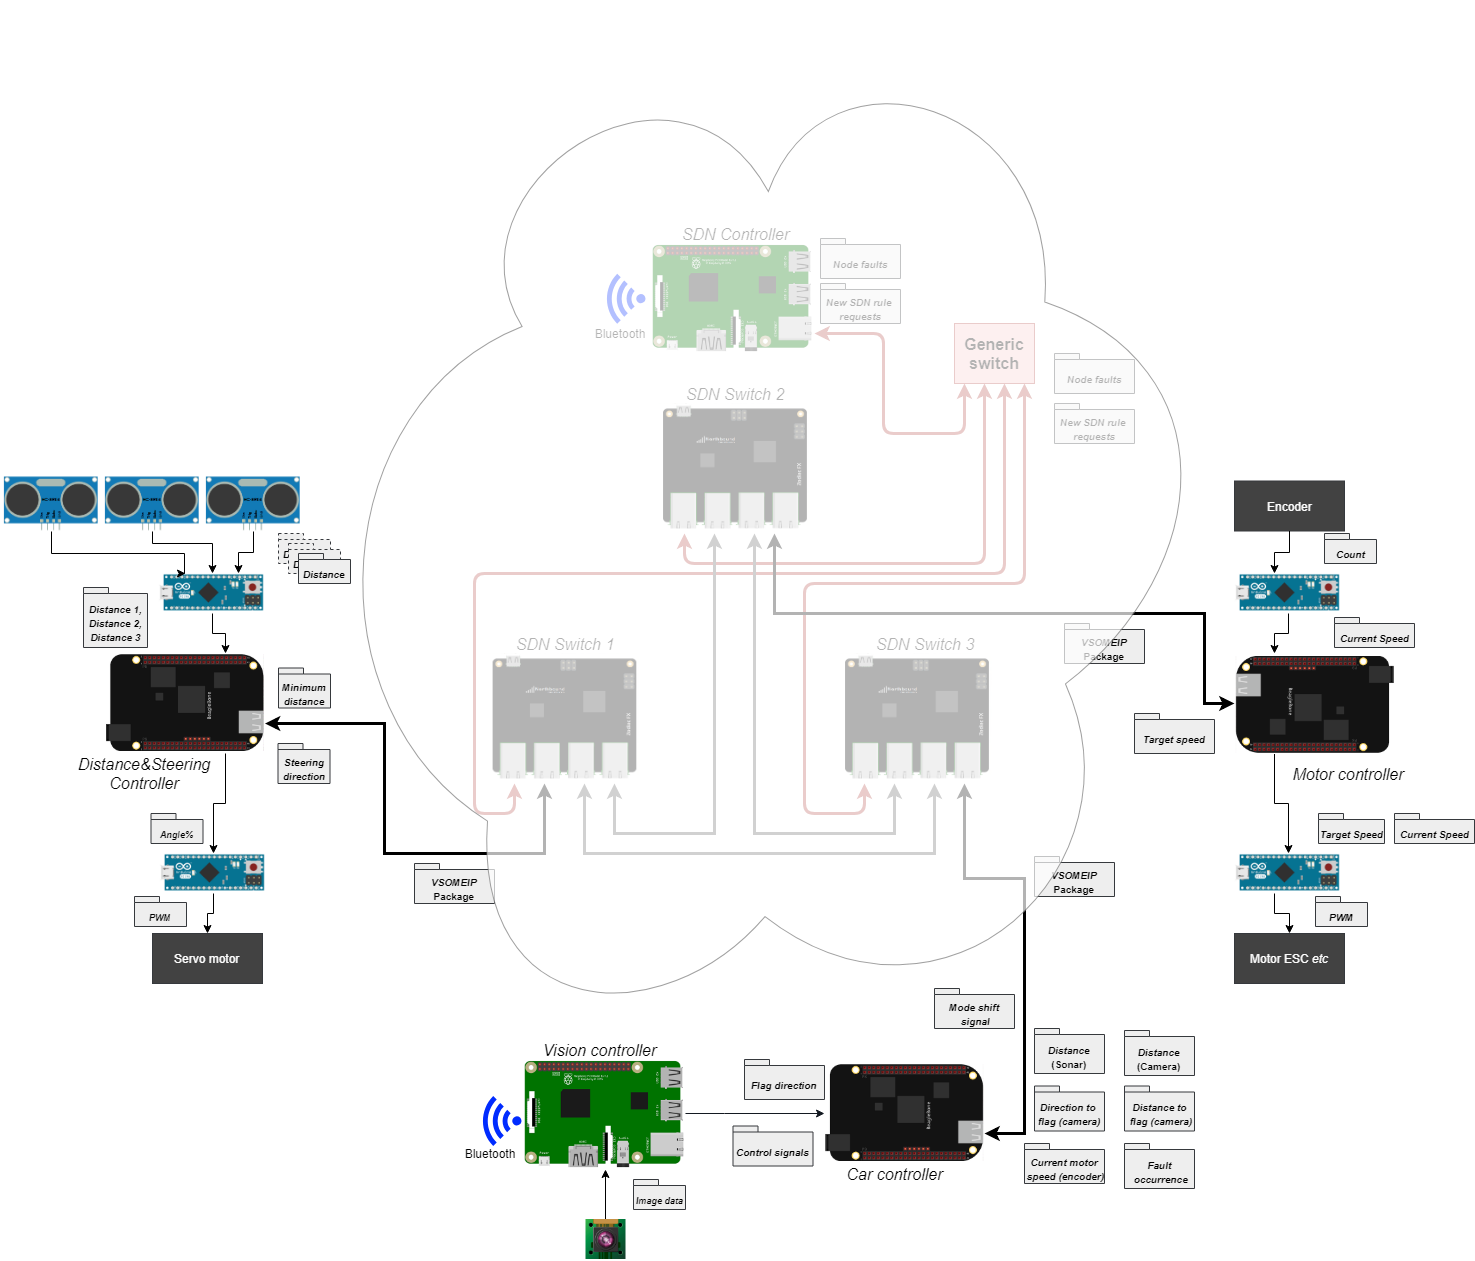
\includegraphics[width=1\linewidth]{network.png}
        \caption{Network topology}
        \label{pic:network}
        \end{figure}
    
\end{block}

%----------------------------------------------------------------------------------------
%	Control and Sensors 
%----------------------------------------------------------------------------------------

\begin{block}{Control and sensors}

\begin{itemize}
    \item On the car is three ultrasound sensors placed to detect object in front of the car, to give information to the controller if something is in front of it. Three sensors was used to detect obstacle from left, right and in the middle of the car direction
    
    \item The car should be able to detect traffic signs, and we did a simplification of only using colours to drive the car. If there is a green signed in front of the car will it follow it and if the sign is red it will stop.  
    
    \item Speed sensor
\end{itemize}

\end{block}

%----------------------------------------------------------------------------------------
%	
%----------------------------------------------------------------------------------------



%----------------------------------------------------------------------------------------

\end{column} % End of the first column

\begin{column}{.03\textwidth}\end{column} % Empty spacer column
 
\begin{column}{.465\textwidth} % The second column
    \begin{block}{Assembley}

        \begin{itemize}
            \item The car was assembled via via some acyle plastic that was used to cut out the pieces to assemble the devices one the car.
            \item The design of the assembly platform is done in Autodesk fusion 360
            
            
            \item The car is power via a lithium battery of 3 cells and is used power the engine and all the components of the car. The power is deliver from the PCB designs and via a boost converter to boost the 5v to 9v to run one of the switches.
              
        \end{itemize}
    
    \end{block}
%----------------------------------------------------------------------------------------
\begin{block}{Figure of assembely}
    
\end{block}

%------------------------------------------------

\





%----------------------------------------------------------------------------------------
%	ACKNOWLEDGEMENTS
%----------------------------------------------------------------------------------------

\begin{block}{Acknowledgments}

\begin{itemize}
\item We want to thank the project owners for their support they have given us under this project. 
\end{itemize}

\end{block}

%----------------------------------------------------------------------------------------
%	CONTACT INFORMATION
%----------------------------------------------------------------------------------------

\setbeamercolor{block title}{fg=black,bg=orange!70} % Change the block title color

\begin{block}{Prodject Information}

\begin{itemize}
\item Github: \href{https://github.com/fhyy/MF2063-ESS-NW-CAR}{https://github.com/fhyy/MF2063-ESS-NW-CAR}

\end{itemize}

\end{block}

%----------------------------------------------------------------------------------------

\end{column} % End of the second column

\begin{column}{.015\textwidth}\end{column} % Empty spacer column

\end{columns} % End of all the columns in the poster

\end{frame} % End of the enclosing frame

\end{document}